%\maketitle

\tableofcontents

\newpage

\section{Задание}
\subsection{Условие}
По выданному преподавателем варианту разработать и исследовать работу комплекса программ обмена данными в режиме прерывания программы. Основная программа должна изменять содержимое заданной ячейки памяти (Х), которое должно быть представлено как знаковое число. Область допустимых значений изменения Х должна быть ограничена заданной функцией F(X) и конструктивными особенностями регистра данных ВУ (8-ми битное знаковое представление). Программа обработки прерывания должна выводить на ВУ модифицированное значение Х в соответствии с вариантом задания, а также игнорировать все необрабатываемые прерывания.

\begin{figure}[H]
\centering
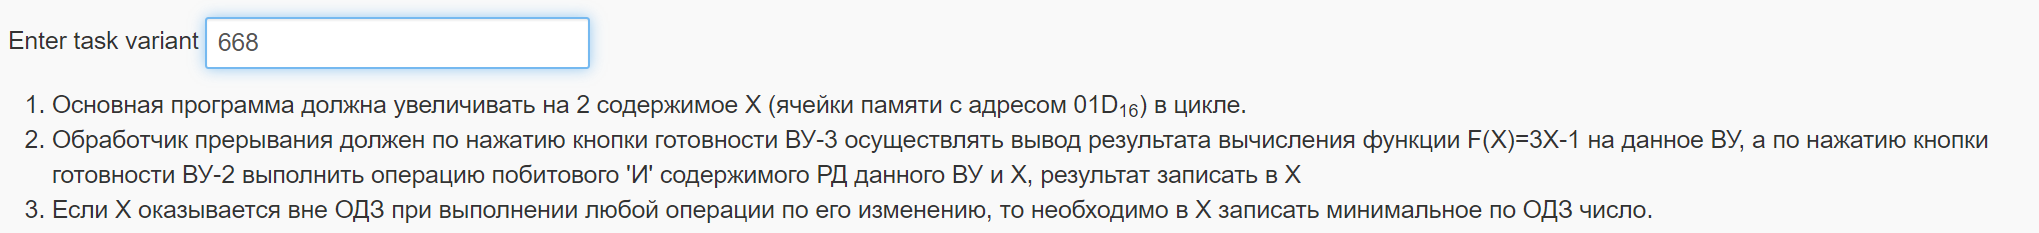
\includegraphics[scale=0.33]{task}
\label{pic:task}
\end{figure}



\newpage
\section{Текст программы}
\noindent\begin{center}
	\begin{tabular}{l}
		\begin{lstlisting}[basicstyle=\ttfamily]
	   ORG 0x0	; §Блок §инициализации§ векторов§
VECTOR_0:  WORD $DEF_HAND, 0x180 ; прерывания§
VECTOR_1:  WORD $DEF_HAND, 0x180
VECTOR_2:  WORD $INT2, 0x180
VECTOR_3:  WORD $INT3, 0x180
VECTOR_4:  WORD $DEF_HAND, 0x180
VECTOR_5:  WORD $DEF_HAND, 0x180
VECTOR_6:  WORD $DEF_HAND, 0x180
VECTOR_7:  WORD $DEF_HAND, 0x180
	
DEF_HAND:  PUSH	; Дефолтный §обработчик §прерываний 
ED1_HAND:  IN 3	; §для §ВУ-1§ и §ВУ-4
	   AND #0x40
	   BEQ ED4_HAND
   	   CLA
	   OUT 2

ED4_HAND:  IN 0xA
	   AND #0x40
	   BEQ END_HAND
	   IN 9
		
END_HAND:  POP
	   IRET	

	   ORG 0x1D ; Блок§ инициализации §начального,
X:	   WORD 0 	; §макс.§ и§ мин.§ значений§ X
MIN_X:     WORD 0xFFD6
MAX_X:	   WORD 0x2A

START:	   DI	; Начало§ программы§

INIT_MR:   		; Блок§ привязывания§ MR§ всех§ 
	   LD #8	; КВУ§ к §векторам§ прерывания
	   OUT 3

	   LD #0xA
	   OUT 5
		
	   CLA
	   OUT 6
	
   	   LD #0xB 
	   OUT 7
		
	   LD #9
	   OUT 0xB
		
EXEC:	   EI	; Начало§ основного§ цикла
	   NOP	;
	
OPER:	   DI	; Блок§ операции§ увеличения§ X§ на§ 2§ 
	   LD X	;§ и§ сохранения§ результата§ по §адресу §X,
	   ADD #0x2	;§ если§ X §превысит§ MAX_X,§ 
	   CMP MAX_X	;§ то §X §будет§ присвоено§ MIN_X
		
			   
		\end{lstlisting}
	\end{tabular}
\end{center}

\newpage
\noindent\begin{center}
	\begin{tabular}{l}
		\begin{lstlisting}[basicstyle=\ttfamily]
	   ST TMP_X_MID	; Сохранение§ промежуточных§ 
	   PUSHF	; X §и§ PS
	   LD &0
	   ST TMP_PS_MID
	   LD TMP_X_MID
	   POPF
	
	   BLT SAVE_X
	   BEQ SAVE_X
	   LD MIN_X
		
SAVE_X:	   ST X
	   PUSHF
	   LD &0
	   ST TMP_PS
	   POPF	; 3F
	
	   LD MAIN_LEN	; Блок §сохранения§ промежуточных§ и  
	   BEQ NEXT	; конечных§ X§ и§ PS§ в §таблицу
	
	   LD TMP_X_MID	; Сохранение §промежуточного§ X
	   ST (MAIN_CUR)+
	
	   LD TMP_PS_MID; Сохранение §промежуточного 
	   ST (MAIN_CUR)+ ; §содержимого§ PS
	
	   LD X
	   ST (MAIN_CUR)+; Сохранение §конечного§ X
	
	   LD TMP_PS; Сохранение§ конечного§
	   ST (MAIN_CUR)+;  содержимого§ PS
	
	   LOOP MAIN_LEN	
	   JUMP NEXT
	   HLT	; БРЕЙКПОИНТ, §для §оставки §после 
		; заполнения§ всей§ отладочной §таблицы
		
NEXT:      EI
	   NOP	; БРЕЙКПОИНТ
	   JUMP OPER	; Зацикливание §увеличения X на 2
	
TMP_X_MID: WORD 0
TMP_PS_MID:WORD 0
TMP_PS:	   WORD 0
	
INT2:	   PUSH	; Блок§ обработчика§ прерывания§ ВУ-2
	   LD X	; Осуществляет§ операцию§ побитого§ И  
	   PUSH	; §содержимого §РДВУ-2§ и§ X, 
		   ; а §результат §присваевает X
			
		\end{lstlisting}
	\end{tabular}
\end{center}

\newpage
\noindent\begin{center}
	\begin{tabular}{l}
		\begin{lstlisting}[basicstyle=\ttfamily]
	   IN 0x4	
	   PUSH
	   AND X	
	   ST X
		
	   CLA
	   IN 5
	   PUSH
		
	   PUSHF
		
	   LD INT2_LEN	; Сохранение§ отладочной§ информации
	   BEQ NEXT_INT2
		
	   LD &3
	   ST (INT2_CUR)+	; Сохранение §начального§ X
	
	   LD &2		; Сохранение§ пользовательского§
	   ST (INT2_CUR)+	;  ввода§ в§ РДВУ-2
		
	   LD X
	   ST (INT2_CUR)+	; Сохранение§ нового §значения§ X
	
	   LD &0
	   ST (INT2_CUR)+	; Сохранение§ содержимого §PS
		
	   LD &1
	   ST (INT2_CUR)+	; Сохранение§ содержимого§ РСВУ-2

	   OR -(INT2_LEN)	
		
NEXT_INT2: POPF
	   POP
	   POP
	   POP
	   POP
	   IRET
		
INT3:      PUSH ; Блок§ обработчика §прерывания§ ВУ-3
	   LD X	; Осуществляет§ подсчет§ функции F(X)=3X-1
	   PUSH	; И§ выводит§ в§ РДВУ-3
	   ASL
	   ADD X
	   DEC
	   OUT 0x6
	   PUSH

	   CLA
	   IN 7
	   PUSH
		
	   PUSHF
		
			   
\end{lstlisting}
\end{tabular}
\end{center}


\newpage
\noindent\begin{center}
	\begin{tabular}{l}
		\begin{lstlisting}[basicstyle=\ttfamily]
		LD INT3_LEN	; Сохранение§ отладочной §информации
		BEQ NEXT_INT3

		LD &3
		ST (INT3_CUR)+	; Сохранение §переменной§ X
	
		LD &2
		ST (INT3_CUR)+	; Сохранение§ результата§ вычисления§ F(X)
		
		LD &0
		ST (INT3_CUR)+	; Сохранение§ содержимого§ PS
		
		LD &1
		ST (INT3_CUR)+	; Сохранение §содержимого§ РСВУ-3
		
		OR -(INT3_LEN)
		
NEXT_INT3:	POPF
		POP
		POP
		POP
		POP
		IRET
		
		ORG 0x90
MAIN_CUR:	WORD $MSTEP_1_X_MID
MAIN_LEN:	WORD 10	; Указывает§ количество §сохранений §в§ таблицу
MSTEP_1_X_MID: WORD 0; Начало §блока§ отладочных§ ячеек 
MSTEP_1_PS_MID: WORD 0;§для §основного§ цикла §программы
MSTEP_1_X: WORD 0
MSTEP_1_PS: WORD 0
MSTEP_2_X_MID: WORD 0
MSTEP_2_PS_MID: WORD 0
MSTEP_2_X: WORD 0
MSTEP_2_PS: WORD 0
MSTEP_3_X_MID: WORD 0
MSTEP_3_PS_MID: WORD 0
MSTEP_3_X: WORD 0
MSTEP_3_PS: WORD 0
MSTEP_4_X_MID: WORD 0
MSTEP_4_PS_MID: WORD 0
MSTEP_4_X: WORD 0
MSTEP_4_PS: WORD 0
MSTEP_5_X_MID: WORD 0
MSTEP_5_PS_MID: WORD 0
MSTEP_5_X: WORD 0
MSTEP_5_PS: WORD 0
MSTEP_6_X_MID: WORD 0
MSTEP_6_PS_MID: WORD 0
MSTEP_6_X: WORD 0
MSTEP_6_PS: WORD 0
MSTEP_7_X_MID: WORD 0
MSTEP_7_PS_MID: WORD 0
MSTEP_7_X: WORD 0
MSTEP_7_PS: WORD 0
MSTEP_8_X_MID: WORD 0
MSTEP_8_PS_MID: WORD 0
MSTEP_8_X: WORD 0
MSTEP_8_PS: WORD 0
MSTEP_9_X_MID: WORD 0
MSTEP_9_PS_MID: WORD 0
MSTEP_9_X: WORD 0
MSTEP_9_PS: WORD 0
		
		\end{lstlisting}
	\end{tabular}
\end{center}
\newpage

\newpage
\noindent\begin{center}
	\begin{tabular}{l}
		\begin{lstlisting}[basicstyle=\ttfamily]
MSTEP_10_X_MID: WORD 0
MSTEP_10_PS_MID: WORD 0
MSTEP_10_X: WORD 0; Конец§ блока §отладочных
MSTEP_10_PS: WORD 0;  §ячеек§ для §основного§ цикла §программы 

INT2_CUR: WORD $INT2STEP_1_X_OLD; Начало §блока §отладочных §ячеек 
INT2_LEN: WORD 5; §для §обработчика §прерываний §ВУ-2
INT2STEP_1_X_OLD: WORD 0
INT2STEP_1_SX: WORD 0
INT2STEP_1_X_NEW: WORD 0
INT2STEP_1_PS: WORD 0
INT2STEP_1_SR: WORD 0
INT2STEP_2_X_OLD: WORD 0
INT2STEP_2_SX: WORD 0
INT2STEP_2_X_NEW: WORD 0
INT2STEP_2_PS: WORD 0
INT2STEP_2_SR: WORD 0
INT2STEP_3_X_OLD: WORD 0
INT2STEP_3_SX: WORD 0
INT2STEP_3_X_NEW: WORD 0
INT2STEP_3_PS: WORD 0
INT2STEP_3_SR: WORD 0
INT2STEP_4_X_OLD: WORD 0
INT2STEP_4_SX: WORD 0
INT2STEP_4_X_NEW: WORD 0
INT2STEP_4_PS: WORD 0
INT2STEP_4_SR: WORD 0
INT2STEP_5_X_OLD: WORD 0
INT2STEP_5_SX: WORD 0
INT2STEP_5_X_NEW: WORD 0
INT2STEP_5_PS: WORD 0; Конец§ блока§ отладочных §ячеек
INT2STEP_5_SR: WORD 0; для§ обработчика§ прерываний§ ВУ-2

INT3_CUR: WORD $INT3STEP_1_X; Начало §блока§ отладочных§ ячеек§ 
INT3_LEN: WORD 5; для §обработчика§ прерываний§ ВУ-3
INT3STEP_1_X: WORD 0
INT3STEP_1_SX: WORD 0
INT3STEP_1_PS: WORD 0
INT3STEP_1_SR: WORD 0
INT3STEP_2_X: WORD 0
INT3STEP_2_SX: WORD 0
INT3STEP_2_PS: WORD 0
INT3STEP_2_SR: WORD 0
INT3STEP_3_X: WORD 0
INT3STEP_3_SX: WORD 0
INT3STEP_3_PS: WORD 0
INT3STEP_3_SR: WORD 0
INT3STEP_4_X: WORD 0
INT3STEP_4_SX: WORD 0
INT3STEP_4_PS: WORD 0
INT3STEP_4_SR: WORD 0
INT3STEP_5_X: WORD 0
INT3STEP_5_SX: WORD 0
INT3STEP_5_PS: WORD 0; Конец §блока §отладочных §ячеек
INT3STEP_5_SR: WORD 0;  §для §обработчика §прерываний §ВУ-3
		\end{lstlisting}
	\end{tabular}
\end{center}
\newpage

\section{Описание программы}
\subsection{Назначение программы}
Увеличение переменной Х на 2 в основной программе в бесконечном цикле. Если переменная Х превысит MAX\_X, то установить X как MIN\_X. При готовности ВУ-3 вывести на РДВУ-3 значение $ F(X) = 3X - 1 $. При готовности ВУ-2 выполнить операцию побитого И содержимого РДВУ-2 и X, а результат сохранить в переменную X.

\subsection{Область представления и область допустимых значений исходных данных и результата}
\subsubsection{Область представления}
\noindent $ X, MAX\_X, MIN\_X $- 8-разрядные знаковые числа с фиксированной запятой. Диапазон значений формата $-2^7\ldots2^7-1$ \\
Содержимое РДВУ-2 - набор из 8 логических значений 1 или 0.

\subsubsection{Область допустимых значений}
\noindent Для вывода результата $ F(X) $ используется 8-битный РДВУ-3, поэтому область значений функции равен $ -2^7\ldots2^7-1 $\\
Или \[ -2^7 \leq 3X - 1 \leq 2^7 -1 \]
\[\frac{-2^7+1}{3}\leq X\leq \frac{2^7}{3}\]
Теперь в нужном формате:
\[D6\leq X\leq 2A\]

\subsection{Расположение в памяти ЭВМ программы, исходных данных и результатов}
\subsubsection{Исходные данные и результат}
\noindent $ X (1D) $ - переменная\\
$90\ldots B9$ - отладочная таблица для основного цикла программы\\
$ BA \ldots  D4$ - отладочная таблица для обработчика прерываний ВУ-2\\
$ D5 \ldots  EA$ - отладочная таблица для обработчика прерываний ВУ-3\\


\subsubsection{Программа}
\noindent$ 0\ldots F $ - блок инициализации векторов прерывания\\
$ 10 \ldots 1B $ - обработчик прерываний по умолчанию\\
$ MIN\_X (1E),MAX\_X0 (1F) $ - константы\\
$ 20\ldots4F $ - основная программа\\
$ 50, 51, 52 $ - локальные переменные\\
$ 53\ldots 70 $ - обработчик прерываний ВУ-2\\
$ 71\ldots8D $ - обработчик прерываний ВУ-3\\


\subsection{Адреса первой и последней исполняемой команд.}
\noindent $ 20 $ - адрес первой исполняемой команды\\

\newpage

\section{Методика проверки}
\subsection{Основная программа}
\noindent Исходные данные: $ X = 20 $\\
Ожидаемое выходное значение X: $ FFDE $\\
\begin{itemize}
	\item Загрузить комплекс программ в БЭВМ
	\item Загрузить в ячейку 1D значение 20 (присвоение $ X = 20 $)
	\item Загрузить в ячейку 91 значение A (присвоение $ MAIN\_LEN = A $)
	\item Проверить наличие команды HLT по адресу 4C
	\item Запустить программу и дождаться ее остановки
	\item Если программа слишком долго работает, то из-за неопределенной внутренней ошибки произошло зацикливание и проверка провалена
	\item Если после остановки программы IP не равен 4D, то проверка провалена
	\item Обратиться к ячейкам памяти $ 92\ldots B9 $ и заполнить таблицу ниже. При наличии расхождений, проверка провалена. Если все сошлось, проверка была осуществлена успешно.
\end{itemize}

\begin{center}
	\begin{tabular}{|c|c|c|c|}
		\hline
		Имя ячейки & Адрес ячейки & Значение после проверки & Ожидаемое значение \\
		\hline \hline
		MSTEP\_1\_X\_MID  & 92 &    & 0022 \\ \hline
		MSTEP\_1\_PS\_MID & 93 &  & 0188 \\\hline
		MSTEP\_1\_X & 94 &  & 0022 \\\hline
		MSTEP\_1\_PS & 95 &  & 0188 \\\hline
		MSTEP\_2\_X\_MID & 96 &  & 0024 \\\hline
		MSTEP\_2\_PS\_MID & 97 &  & 0188 \\\hline
		MSTEP\_2\_X & 98 &  & 0024 \\\hline
		MSTEP\_2\_PS & 99 &  & 0188 \\\hline
		MSTEP\_3\_X\_MID & 9A &  & 0026 \\\hline
		MSTEP\_3\_PS\_MID & 9B &  & 0188 \\\hline
		MSTEP\_3\_X & 9C &  & 0026 \\\hline
		MSTEP\_3\_PS & 9D &  & 0188 \\\hline
		MSTEP\_4\_X\_MID & 9E &  & 0028 \\\hline
		MSTEP\_4\_PS\_MID & 9F &  & 0188 \\\hline
		MSTEP\_4\_X & A0 &  & 0028 \\\hline
		MSTEP\_4\_PS & A1 &  & 0188 \\\hline
		MSTEP\_5\_X\_MID & A2 &  & 002A \\\hline
		MSTEP\_5\_PS\_MID & A3 &  & 0185 \\\hline
		MSTEP\_5\_X & A4 &  & 002A \\\hline
		MSTEP\_5\_PS & A5 &  & 0185 \\\hline
		MSTEP\_6\_X\_MID & A6 &  & 002C \\\hline
		MSTEP\_6\_PS\_MID & A7 &  & 0181 \\\hline
		MSTEP\_6\_X & A8 &  & FFD6 \\\hline
		MSTEP\_6\_PS & A9 &  & 0189 \\\hline
		MSTEP\_7\_X\_MID & AA &  & FFD8 \\\hline
		MSTEP\_7\_PS\_MID & AB &  & 0189 \\\hline
		MSTEP\_7\_X & AC &  & FFD8 \\\hline
		MSTEP\_7\_PS & AD &  & 0189 \\\hline
		MSTEP\_8\_X\_MID & AE &  & FFDA \\\hline
		MSTEP\_8\_PS\_MID & AF &  & 0189 \\\hline
		MSTEP\_8\_X & B0 &  & FFDA \\\hline
		MSTEP\_8\_PS & B1 &  & 0189 \\\hline
		MSTEP\_9\_X\_MID & B2 &  & FFDC \\\hline
		MSTEP\_9\_PS\_MID & B3 &  & 0189 \\\hline
		MSTEP\_9\_X & B4 &  & FFDC \\\hline
		MSTEP\_9\_PS & B5 &  & 0189 \\\hline
		MSTEP\_10\_X\_MID & B6 &  & FFDE \\\hline
		MSTEP\_10\_PS\_MID & B7 &  & 0189 \\\hline
		MSTEP\_10\_X & B8 &  & FFDE \\\hline
		MSTEP\_10\_PS & B9 &  & 0189 \\\hline
		\hline
	\end{tabular}
\end{center}

\newpage
\subsection{Обработчик ВУ-2}
\noindent Исходные данные: $ X = 20 $\\
Значение 1: FF\\
Значение 2: BA\\
Значение 3: E9\\
Значение 4: DE\\
Значение 5: AD\\

\begin{itemize}
	\item Загрузить комплекс программ в БЭВМ
	\item Загрузить в ячейку 1D значение 20 (присвоение $ X = 20 $)
	\item Загрузить в ячейку 91 значение A (присвоение $ MAIN\_LEN = A $)
	\item Загрузить в ячейку BB значение 5 (присвоение $ INT2\_LEN = 5 $)
	\item Проверить наличие команды HLT по адресу 4C
	\item Запустить программу
	\item Записать в ВУ-2 "Значение 1" и установить "Готовность ВУ-2"
	\item Дождаться отмены "готовности ВУ-2"
	\item Повторить предыдушие 2 шага еще 4 раза, каждый раз используя новое "Значение"
	\item Дождаться остановки программы
	\item Если программа слишком долго работает, то из-за неопределенной внутренней ошибки произошло зацикливание и проверка провалена
	\item Если после остановки программы IP не равен 4D, то проверка провалена
	\item Обратиться к ячейкам памяти $ BC\ldots D4 $ и заполнить таблицу ниже. При наличии расхождений, проверка провалена. Ячейки с прочерком подразумевают трудно предсказуемый результат, поэтому проверяющему нужно самому осуществить операцию побитового "И" X\_OLD и SX, а после сравнить с X\_NEW. Если SR не равно ожидаемому значению, то можно предположить что проверяющий слишком часто устанавливал "Готовность ВУ-2".
\end{itemize}

\begin{center}
	\begin{tabular}{|c|c|c|c|}
		\hline
		Имя ячейки & Адрес ячейки & Значение после проверки & Ожидаемое значение \\
		\hline \hline
		INT2STEP\_1\_X\_OLD & BC &  & --- \\\hline
		INT2STEP\_1\_SX & BD &  & 00FF \\\hline
		INT2STEP\_1\_X\_NEW & BE &  & --- \\\hline
		INT2STEP\_1\_PS & BF &  & --- \\\hline
		INT2STEP\_1\_SR & C0 &  & 0000 \\\hline
		INT2STEP\_2\_X\_OLD & C1 &  & --- \\\hline
		INT2STEP\_2\_SX & C2 &  & 00BA \\\hline
		INT2STEP\_2\_X\_NEW & C3 &  & --- \\\hline
		INT2STEP\_2\_PS & C4 &  & --- \\\hline
		INT2STEP\_2\_SR & C5 &  & 0000 \\\hline
		INT2STEP\_3\_X\_OLD & C6 &  & --- \\\hline
		INT2STEP\_3\_SX & C7 &  & 00E9 \\\hline
		INT2STEP\_3\_X\_NEW & C8 &  & --- \\\hline
		INT2STEP\_3\_PS & C9 &  & --- \\\hline
		INT2STEP\_3\_SR & CA &  & 0000 \\\hline
		INT2STEP\_4\_X\_OLD & CB &  & --- \\\hline
		INT2STEP\_4\_SX & CC &  & 00DE \\\hline
		INT2STEP\_4\_X\_NEW & CD &  & --- \\\hline
		INT2STEP\_4\_PS & CE &  & --- \\\hline
		INT2STEP\_4\_SR & CF &  & 0000 \\\hline
		INT2STEP\_5\_X\_OLD & D0 &  & --- \\\hline
		INT2STEP\_5\_SX & D1 &  & 00AD \\\hline
		INT2STEP\_5\_X\_NEW & D2 &  & --- \\\hline
		INT2STEP\_5\_PS & D3 &  & --- \\\hline
		INT2STEP\_5\_SR & D4 &  & 0000 \\\hline
		
		\hline
	\end{tabular}
\end{center}

\newpage
\subsection{Обработчик ВУ-3}
\noindent Исходные данные: $ X = 20 $\\

\begin{itemize}
	\item Загрузить комплекс программ в БЭВМ
	\item Загрузить в ячейку 1D значение 20 (присвоение $ X = 20 $)
	\item Загрузить в ячейку 91 значение A (присвоение $ MAIN\_LEN = A $)
	\item Загрузить в ячейку D6 значение 5 (присвоение $ INT3\_LEN = 5 $)
	\item Проверить наличие команды HLT по адресу 4C
	\item Запустить программу
	\item Установить "Готовность ВУ-3"
	\item Дождаться отмены "готовности ВУ-3"
	\item Повторить предыдушие 2 шага еще 4 раза
	\item Дождаться остановки программы
	\item Если программа слишком долго работает, то из-за неопределенной внутренней ошибки произошло зацикливание и проверка провалена
	\item Если после остановки программы IP не равен 4D, то проверка провалена
	\item Обратиться к ячейкам памяти $ D7\ldots EA $ и заполнить таблицу ниже. При наличии расхождений, проверка провалена. Ячейки с прочерком подразумевают трудно предсказуемый результат, поэтому проверяющему нужно самому подсчитать значение F(X) для X и сравнить со значением в SX. Если SR не равно ожидаемому значению, то можно предположить что проверяющий слишком часто устанавливал "Готовность ВУ-3".
\end{itemize}

\begin{center}
	\begin{tabular}{|c|c|c|c|}
		\hline
		Имя ячейки & Адрес ячейки & Значение после проверки & Ожидаемое значение \\
		\hline \hline
		INT3STEP\_1\_X & D7 &  & --- \\\hline
		INT3STEP\_1\_SX & D8 &  & --- \\\hline
		INT3STEP\_1\_PS & D9 &  & --- \\\hline
		INT3STEP\_1\_SR & DA &  & 0000 \\\hline
		INT3STEP\_2\_X & DB &  & --- \\\hline
		INT3STEP\_2\_SX & DC &  & --- \\\hline
		INT3STEP\_2\_PS & DD &  & --- \\\hline
		INT3STEP\_2\_SR & DE &  & 0000 \\\hline
		INT3STEP\_3\_X & DF &  & --- \\\hline
		INT3STEP\_3\_SX & E0 &  & --- \\\hline
		INT3STEP\_3\_PS & E1 &  & --- \\\hline
		INT3STEP\_3\_SR & E2 &  & 0000 \\\hline
		INT3STEP\_4\_X & E3 &  & --- \\\hline
		INT3STEP\_4\_SX & E4 &  & --- \\\hline
		INT3STEP\_4\_PS & E5 &  & --- \\\hline
		INT3STEP\_4\_SR & E6 &  & 0000 \\\hline
		INT3STEP\_5\_X & E7 &  & --- \\\hline
		INT3STEP\_5\_SX & E8 &  & --- \\\hline
		INT3STEP\_5\_PS & E9 &  & --- \\\hline
		INT3STEP\_5\_SR & EA &  & 0000 \\\hline
		
		
		\hline
	\end{tabular}
\end{center}

\newpage
\subsection{Обработчик по умолчанию}

\begin{itemize}
	\item Загрузить комплекс программ в БЭВМ
	\item Проверить наличие команды HLT по адресу 4C
	\item Запустить программу
	\item Установить "Готовность ВУ-1"
	\item Дождаться сброса "Готовность ВУ-1", если этого не происходит длительное время, программа зациклена, проверка провалена.
\end{itemize}

Проверить ВУ-4 не представляется возможным, ибо при нажатии на соответсвующую кнопку ВУ-4 не открывается.

\section{Вывод}
В ходе выполнения лабораторной работы я изучил организацию ввода-вывода при помощи прерываний в БЭВМ, разработал программу, в которой реализовал тривиальные обработчики прерываний, а также разработал методику проверки работоспособности своей работы.
